\section{Appendix} % (fold)
\label{sec:appendix}


\subsection{Tables} % (fold)
\label{sub:tables}

\begin{table}[!h]
\centering
\caption{Variable Descriptions}
\label{my-label}
\begin{adjustbox}{angle=90}
\begin{tabular}{llll}
Full dataset  &                                                                                                                 &                   &           \\
Variable Name & Variable Description                                                                                            & Example           & Dimension \\
NEWID         & NEWID is the variable inditcating each individual houseld survey                                                & 1292531           & 44746*1   \\
UCC           & UCC represents each products unique universal classification code                                               & 10120             & 548*1     \\
Description   & Description describes each individual product                                                                   & Savings acc.      &           \\
N             & The amount of times a product was purchsed by a particular household                                            & 1                 & 1195829*1 \\
Gift          & Gifts represents whether a household purchased a gift or not & 1,0               & 44746*1   \\
AGE           & The average age of a household                                                                                  & 67                & 44746*1   \\
EDUCA         & The maximum level of education within a household                                                               & 8                 & 44746*1   \\
STATE         & The state in which the survey was conducted                                                                     & 51                & 44746*1   \\
SEX           & Whether the household is male or female dominated, or balanced.                                                 & M                 & 44746*1   \\
INCLASS       & The inclome class of the household                                                                              & \textgreater75000 & 44746*1  
\end{tabular}
\end{adjustbox}
\end{table}



% subsection tables (end)
\clearpage



\subsection{Figures} % (fold)
\label{sub:figures}

\begin{figure}[!h]
\caption{Top 10 Words Over 7 Topics}\centering
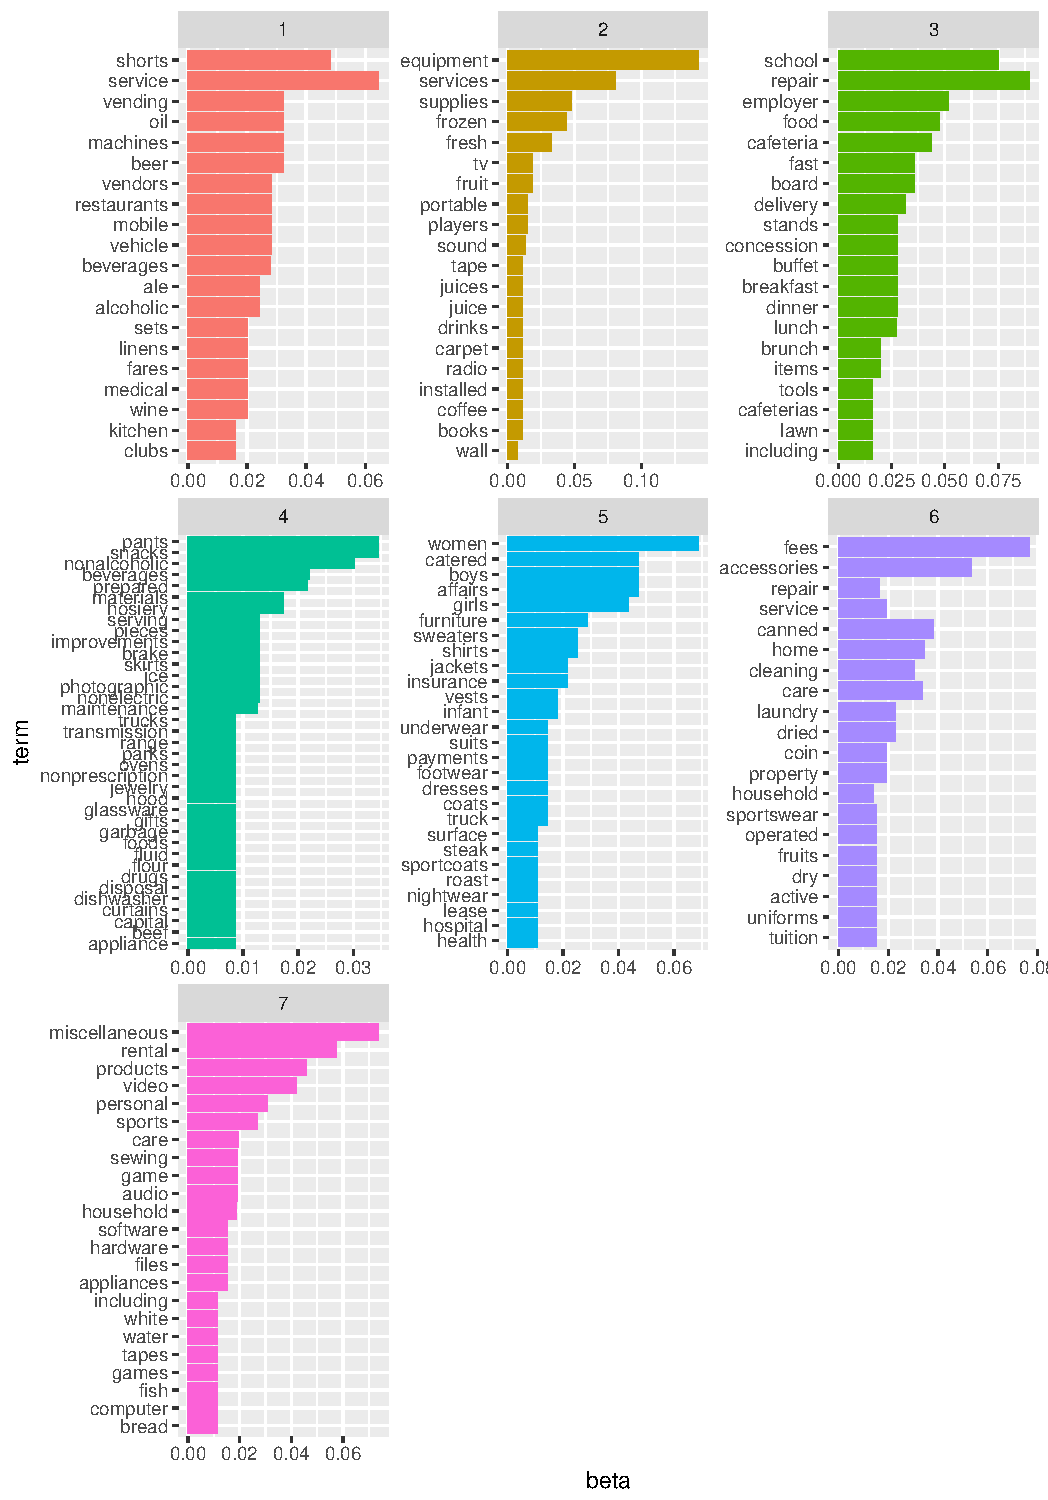
\includegraphics[width=1\textwidth]{/Users/charlvanschoor/Documents/Gottingen/ML/ML-Applications-CVS/LDA_consumer_analysis/paper/content/graphs/topicsper30_before_wiki.pdf}
\end{figure}
\begin{figure}
\caption{Word-Count Per Product}\centering
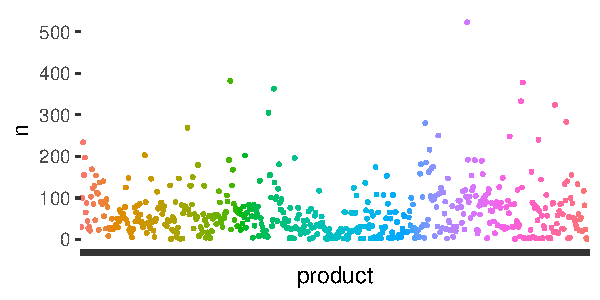
\includegraphics[width=1.1\textwidth]{/Users/charlvanschoor/Documents/Gottingen/ML/ML-Applications-CVS/LDA_consumer_analysis/paper/content/graphs/word-count-per-product.pdf}
\end{figure}

\begin{figure}
\caption{CPP Matrix Visualization}\centering
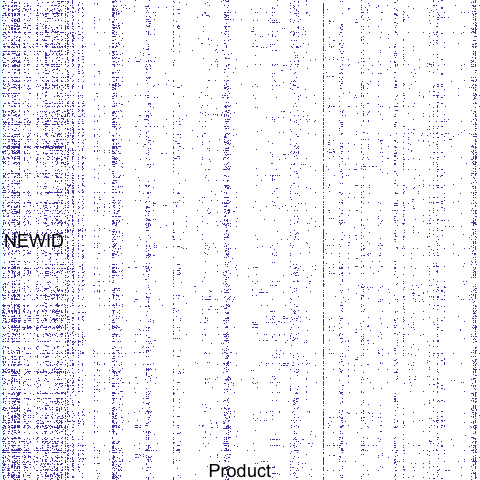
\includegraphics[width=1.1\textwidth]{/Users/charlvanschoor/Documents/Gottingen/ML/ML-Applications-CVS/LDA_consumer_analysis/src/output/CPP-distribution/CPP_distribution.png}
\end{figure}



\begin{figure}
\caption{Distribution of Household Age for Gift and Non-Gift}\centering
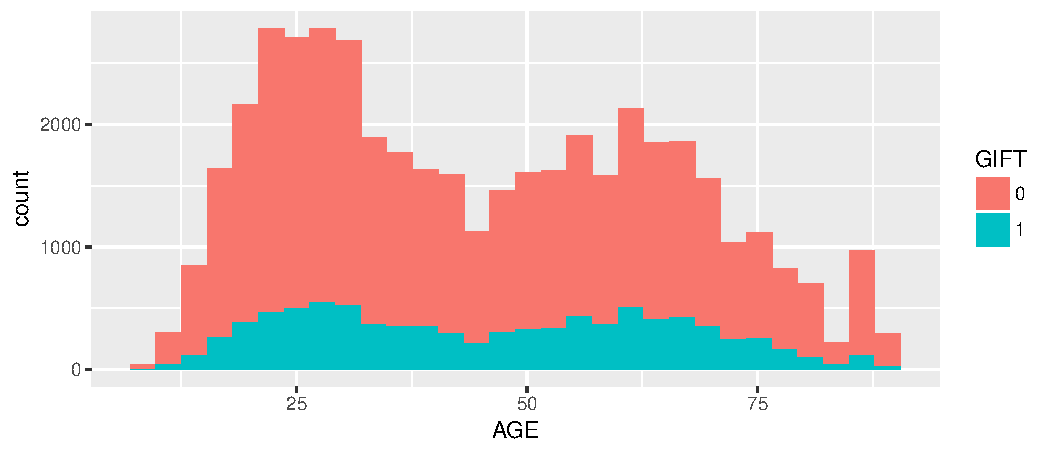
\includegraphics[width=1.1\textwidth]{/Users/charlvanschoor/Documents/Gottingen/ML/ML-Applications-CVS/LDA_consumer_analysis/src/output/CES-distributions/AGE.pdf}
\end{figure}

\begin{figure}
\caption{Distribution of Household Sex for Gift and Non-Gift}\centering
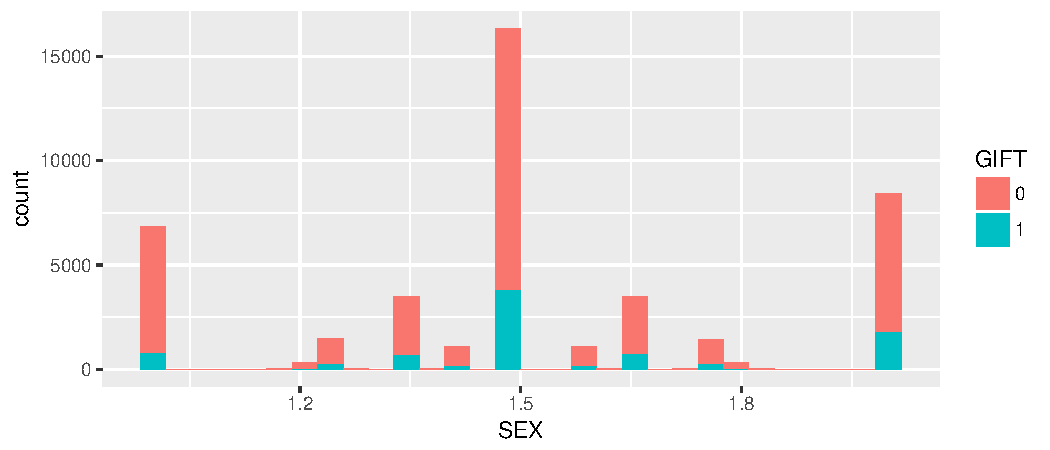
\includegraphics[width=1.1\textwidth]{/Users/charlvanschoor/Documents/Gottingen/ML/ML-Applications-CVS/LDA_consumer_analysis/src/output/CES-distributions/SEX.pdf}
\end{figure}

\begin{figure}
\caption{Distribution of Household Education for Gift and Non-Gift}\centering
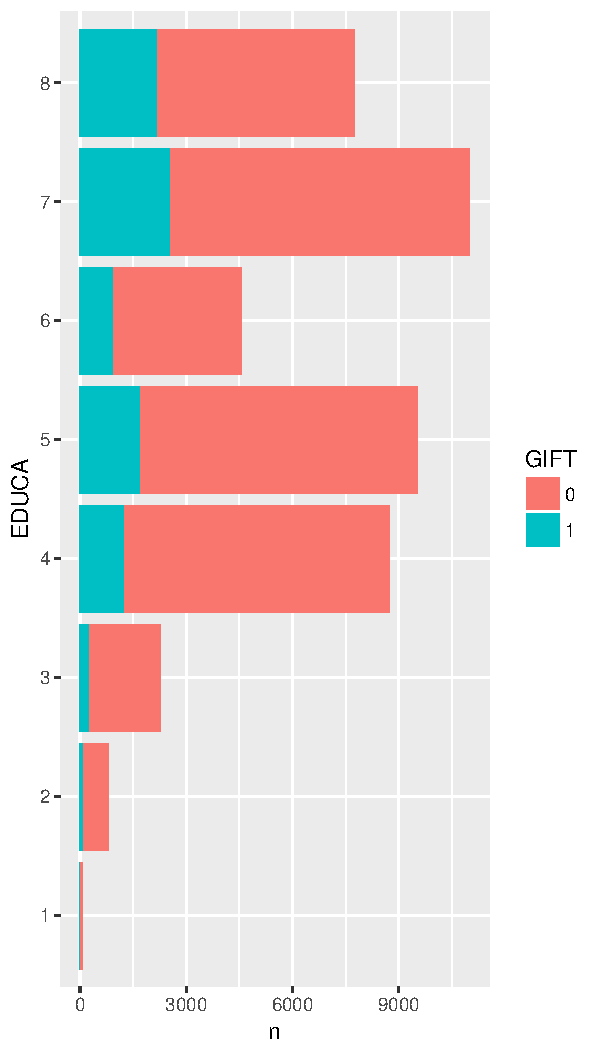
\includegraphics[width=0.8\textwidth]{/Users/charlvanschoor/Documents/Gottingen/ML/ML-Applications-CVS/LDA_consumer_analysis/src/output/CES-distributions/EDUCA.pdf}
\end{figure}

\begin{figure}
\caption{Distribution of Household Income Class for Gift and Non-Gift}\centering
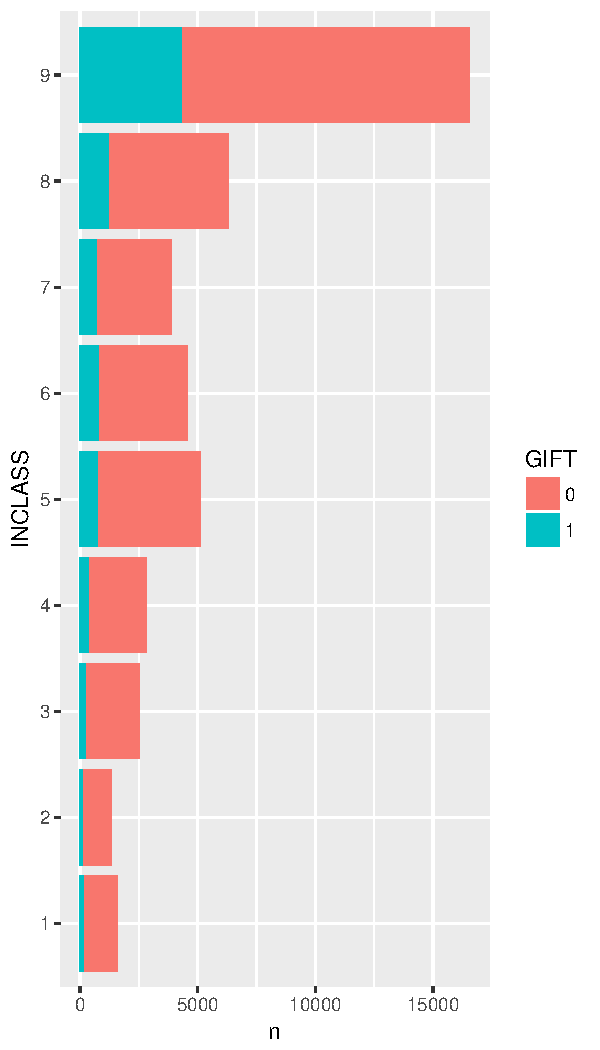
\includegraphics[width=0.8\textwidth]{/Users/charlvanschoor/Documents/Gottingen/ML/ML-Applications-CVS/LDA_consumer_analysis/src/output/CES-distributions/INCLASS.pdf}
\end{figure}



\begin{figure}
\caption{Distribution of State for Gift and Non-Gift}\centering
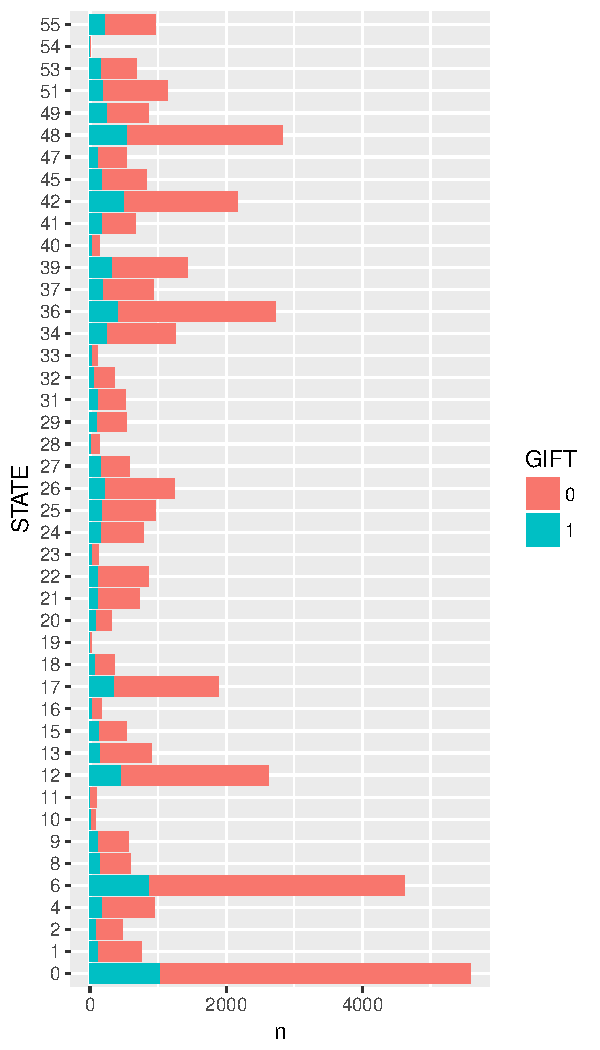
\includegraphics[width=0.8\textwidth]{/Users/charlvanschoor/Documents/Gottingen/ML/ML-Applications-CVS/LDA_consumer_analysis/src/output/CES-distributions/STATE.pdf}
\end{figure}


% subsection figures (end)




% section appendix (end)